\section{Arithmetik}
\subsection{addieren und subtrahieren}
Addieren und Subtrahieren benötigt keine Fallunterscheidung, solange sich die 
negative Zahl im Zweierkomplement befindet.\\
Es gilt:\\
\begin{table}[h]
\begin{tabular}{ll|l}

MSB & LSB & Resalt \\ \hline
0   & 0   & 0      \\ 
0   & 1   & 1      \\ 
1   & 0   & 1      \\ 
1   & 1   & 0      \\ 
\end{tabular}
\end{table}

\noindent Man muss sich bewusst sein, das Resultat von einer Adition liegt im 
normalen Binärsystem vor. Das Resultat bei einer Addition von negativen Zahlen 
die im Zweierkomplement verrechnet wurden, liegt auch das Resultat im 
Zweierkomplement vor.

\subsection{Zweierkomplement}
Sobald eine vorzeichenbelastete binäre Zahlenvektor zu verarbeiten ist, muss 
das MSB betrachtet werden.\\
Ist das MSB eine 0 ist der Zahlenvektor postiv. Hat der Zahlenvektor eine 1 
als MSB so handelt ich es um einen neagtiven Wert.
\\
Negative binär Werte mussen ins Zweierkomplement gewandelt werden.\\
Vorgenhen:\\
Alle Bits invertieren und beim LSB eine 1 dazu addieren.
\\
Um aus dem Zweierkomplement wieder auf einen normalen binären Bitvektor zu 
gelangen wird das Selbe gemacht\\
Alle Bits invertieren und beim LSB eine 1 dazu addieren.
\begin{figure}[htbp]
	\centering
		\includegraphics[width=6cm]{content/bilder/Zahlenkreis.png}
	\caption{Vier Bit signed Zahlenkreis Dezimal und Zweierkomplement Angabe}%
	\label{Zahlenkreis}
\end{figure}

\subsection{Umwandlung signed / unsigned}
\begin{figure}[h!]
    \centering
    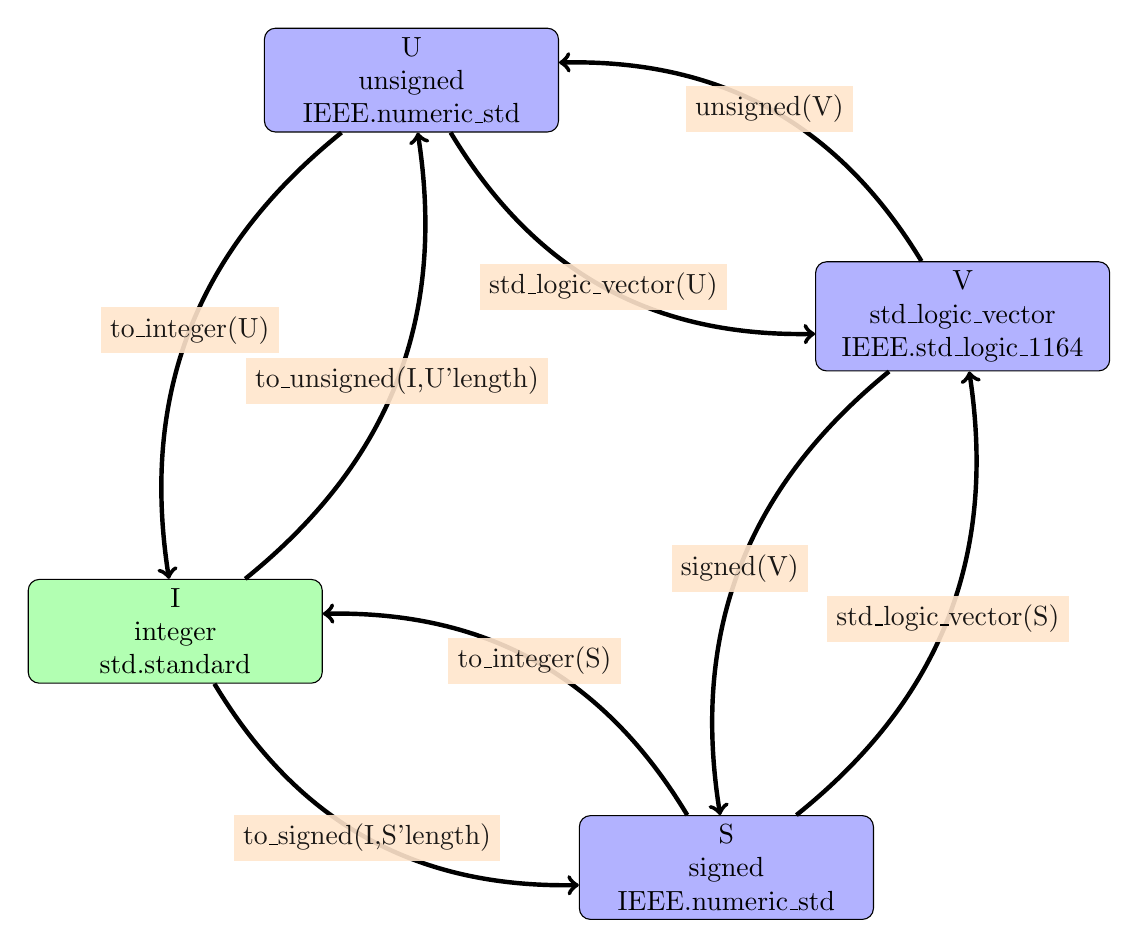
\begin{tikzpicture}
        \node (V) at ( 5, 2) [rounded corners, draw, text width=3.5cm, align=center, fill=blue!30 ] {V\\std\_logic\_vector\\IEEE.std\_logic\_1164};
        \node (U) at (-2, 5) [rounded corners, draw, text width=3.5cm, align=center, fill=blue!30 ] {U\\unsigned\\IEEE.numeric\_std};
        \node (I) at (-5,-2) [rounded corners, draw, text width=3.5cm, align=center, fill=green!30] {I\\integer\\std.standard};
        \node (S) at ( 2,-5) [rounded corners, draw, text width=3.5cm, align=center, fill=blue!30 ] {S\\signed\\IEEE.numeric\_std};

        % V -> U
        \draw[->, ultra thick] (V) to[bend right=30] node[fill=orange!20, fill opacity=0.9] {unsigned(V)} (U);
        % U -> V
        \draw[->, ultra thick] (U) to[bend right=30] node[fill=orange!20, fill opacity=0.9] {std\_logic\_vector(U)} (V);
        % I -> U
        \draw[->, ultra thick] (I) to[bend right=30] node[fill=orange!20, fill opacity=0.9] {to\_unsigned(I,U'length)} (U);
        % U -> I
        \draw[->, ultra thick] (U) to[bend right=30] node[fill=orange!20, fill opacity=0.9] {to\_integer(U)} (I);
        % I -> S
        \draw[->, ultra thick] (I) to[bend right=30] node[fill=orange!20, fill opacity=0.9] {to\_signed(I,S'length)} (S);
        % S -> I
        \draw[->, ultra thick] (S) to[bend right=30] node[fill=orange!20, fill opacity=0.9] {to\_integer(S)} (I);
        % V -> S
        \draw[->, ultra thick] (V) to[bend right=30] node[fill=orange!20, fill opacity=0.9] {signed(V)} (S);
        % S -> V
        \draw[->, ultra thick] (S) to[bend right=30] node[fill=orange!20, fill opacity=0.9] {std\_logic\_vector(S)} (V);
    \end{tikzpicture}
\end{figure}
